\documentclass[border=3pt,tikz]{standalone}
% Shared look for every TikZ figure in these notes.
% Included by each standalone figure file; also keeps the figures consistent
% with the colours used in the PDF and on the website.

\usepackage{tikz}
\usepackage{pgfplots}
\pgfplotsset{compat=1.18}
\usetikzlibrary{arrows.meta, decorations.markings, decorations.pathmorphing,
                patterns, calc, positioning}
\usepackage{amsmath}

% Series colours are the three validated categorical slots also used by the
% interactive widgets, so a path drawn in the printed notes and the same path on
% the website are the same colour. They clear the colour-vision-deficiency and
% contrast checks as a set; every path is direct-labelled as well, so colour is
% never the only thing carrying identity.
\definecolor{duPurple}{HTML}{68246D}
\definecolor{duBlue}{HTML}{2A78D6}
\definecolor{duRed}{HTML}{EB6834}
\definecolor{duGreen}{HTML}{1BAF7A}
\definecolor{duGrey}{HTML}{6B6B6B}

\tikzset{
  axisline/.style   = {-{Stealth[length=3mm]}, line width=0.7pt, black},
  path1/.style      = {duBlue,   line width=1.1pt},
  path2/.style      = {duRed,    line width=1.1pt},
  path3/.style      = {duGreen,  line width=1.1pt},
  statedot/.style   = {circle, fill=black, inner sep=1.4pt},
  arrowhead/.style  = {decoration={markings,
                        mark=at position #1 with {\arrow{Stealth[length=2.6mm]}}},
                       postaction={decorate}},
  lbl/.style        = {font=\small},
  slbl/.style       = {font=\footnotesize, duGrey},
  workfill/.style   = {duPurple, opacity=0.16},
}

\begin{document}
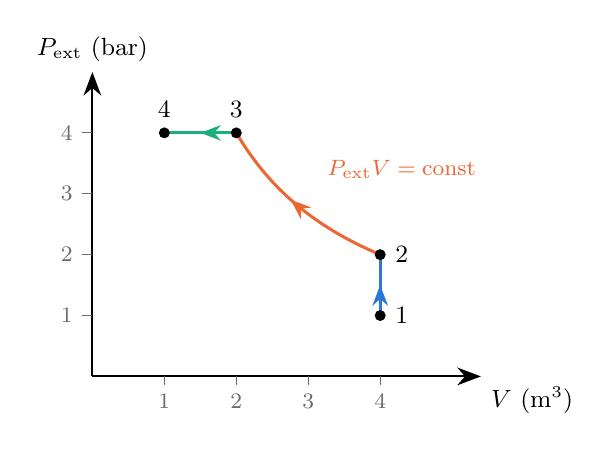
\begin{tikzpicture}[x=26pt, y=22pt]
  \draw[axisline] (0,0) -- (5.4,0) node[below right, lbl] {$V$ (m$^3$)};
  \draw[axisline] (0,0) -- (0,5.0) node[above, lbl] {$P_\text{ext}$ (bar)};

  % 1 (4 m3, 1 bar) -> 2 (4, 2) -> 3 (2, 4) along PV = const -> 4 (1, 4)
  \draw[path1, arrowhead=0.5] (4,1) -- (4,2);
  \draw[path2, arrowhead=0.55] plot[domain=4:2, samples=60] (\x, {8/\x});
  \draw[path3, arrowhead=0.5] (2,4) -- (1,4);

  \node[statedot] at (4,1) {}; \node[lbl, right=2pt] at (4,1) {1};
  \node[statedot] at (4,2) {}; \node[lbl, right=2pt] at (4,2) {2};
  \node[statedot] at (2,4) {}; \node[lbl, above=2pt] at (2,4) {3};
  \node[statedot] at (1,4) {}; \node[lbl, above=2pt] at (1,4) {4};

  \foreach \v in {1,2,3,4} {\draw[duGrey, line width=0.4pt] (\v,0) -- (\v,-0.14);
    \node[slbl, below] at (\v,-0.14) {\v};}
  \foreach \yy in {1,2,3,4} {\draw[duGrey, line width=0.4pt] (0,\yy) -- (-0.14,\yy);
    \node[slbl, left] at (-0.14,\yy) {\yy};}

  \node[slbl, duRed, align=left] at (4.3,3.4) {$P_\text{ext}V=\text{const}$};
\end{tikzpicture}
\end{document}
